\documentclass[10pt, aspectratio=169]{beamer}
% Shared setup for every day of the course.
\usetheme[progressbar=frametitle, numbering=fraction, block=fill]{metropolis}
\usepackage[T1]{fontenc}
\usepackage[utf8]{inputenc}
\usepackage{lmodern}
\usepackage{amsmath, amssymb, bm, booktabs, graphicx, xcolor}
\usepackage{tikz}
\usetikzlibrary{arrows.meta, positioning, calc, shapes.geometric}

\graphicspath{{figures/}}

% --- colours -------------------------------------------------------------------------------------
\definecolor{accent}{HTML}{C0392B}
\definecolor{cool}{HTML}{2E6DB4}
\definecolor{muted}{HTML}{7A7A7A}
\definecolor{good}{HTML}{2E8B57}
\setbeamercolor{alerted text}{fg=accent}
\setbeamercolor{example text}{fg=cool}

% --- notation (follows the thesis' notation chapter) ---------------------------------------------
\newcommand{\given}{\,|\,}
\newcommand{\E}{\mathbb{E}}
\newcommand{\KL}[2]{D_{\mathrm{KL}}\!\left[#1\,\middle\|\,#2\right]}
\newcommand{\N}{\mathcal{N}}
\newcommand{\Hess}{\mathcal{H}}
\newcommand{\nats}{\,\text{nats}}
\DeclareMathOperator*{\argmin}{arg\,min}

% --- course devices ------------------------------------------------------------------------------
% \src{...}: where a claim or number comes from (thesis file and line, or a post-thesis note).
\newcommand{\src}[1]{\par\vfill\hfill{\scriptsize\color{muted}source: #1}}
% \wip: marks a post-thesis result.
\newcommand{\wip}{{\scriptsize\color{white}\colorbox{accent}{\,work in progress\,}}}
% \lesson{...}: the one sentence a frame exists to say.
\newcommand{\lesson}[1]{\begin{alertblock}{}\centering #1\end{alertblock}}
% a measurement story
\newenvironment{measured}[1]{\begin{exampleblock}{Measured: #1}}{\end{exampleblock}}

\author{Course built on the doctoral thesis of No\'e Zapata}
\institute{Montevideo, 30 November -- 4 December 2026}

% \cyclemap{n}: the course's five-stage cycle, stage n highlighted (1 room ... 5 memory).
\newcommand{\cyclemap}[1]{%
  \begin{tikzpicture}[
      st/.style={draw=muted, thick, rounded corners=3pt, fill=white, align=center,
                 minimum width=2.5cm, minimum height=0.8cm, font=\scriptsize, text=muted},
      on/.style={draw=accent, very thick, fill=accent!10, text=black, font=\scriptsize\bfseries},
      arr/.style={-{Stealth[length=2mm]}, thick, color=muted},
      s1/.style={}, s2/.style={}, s3/.style={}, s4/.style={}, s5/.style={}, s#1/.style={on}]
    \node[st, s1] (c1) at (90:1.9)   {estimate the room};
    \node[st, s2] (c2) at (18:2.6)   {localise; learn\\the body};
    \node[st, s3] (c3) at (-54:2.2)  {concepts fill\\the room};
    \node[st, s4] (c4) at (-126:2.2) {cross the door};
    \node[st, s5] (c5) at (162:2.6)  {new room;\\memory};
    \draw[arr] (c1) to[bend left=15] (c2); \draw[arr] (c2) to[bend left=15] (c3);
    \draw[arr] (c3) to[bend left=15] (c4); \draw[arr] (c4) to[bend left=15] (c5);
    \draw[arr] (c5) to[bend left=15] (c1);
  \end{tikzpicture}}


\title{A robot that acts to know}
\subtitle{Day 1 --- The challenge, probability, and free energy}
\date{Monday 30 November}

\begin{document}

\maketitle

% =================================================================================================
\section{The challenge}
% =================================================================================================

\begin{frame}{A robot is put down in an apartment it has never seen}
  \centering
  \vspace{1em}
  {\color{muted}\fbox{\parbox[c][0.55\textheight][c]{0.8\textwidth}{\centering
    \Large [ video: the full cycle, Webots / real apartment ]\\[0.5em]
    \normalsize room estimated $\rightarrow$ localised $\rightarrow$ objects appear
    $\rightarrow$ door crossed $\rightarrow$ second room}}}
  \vspace{1em}

  Watch for one thing: \alert{nothing in this video was programmed as a sequence of steps.}
\end{frame}

\begin{frame}{The cycle we will build this week}
  \centering
  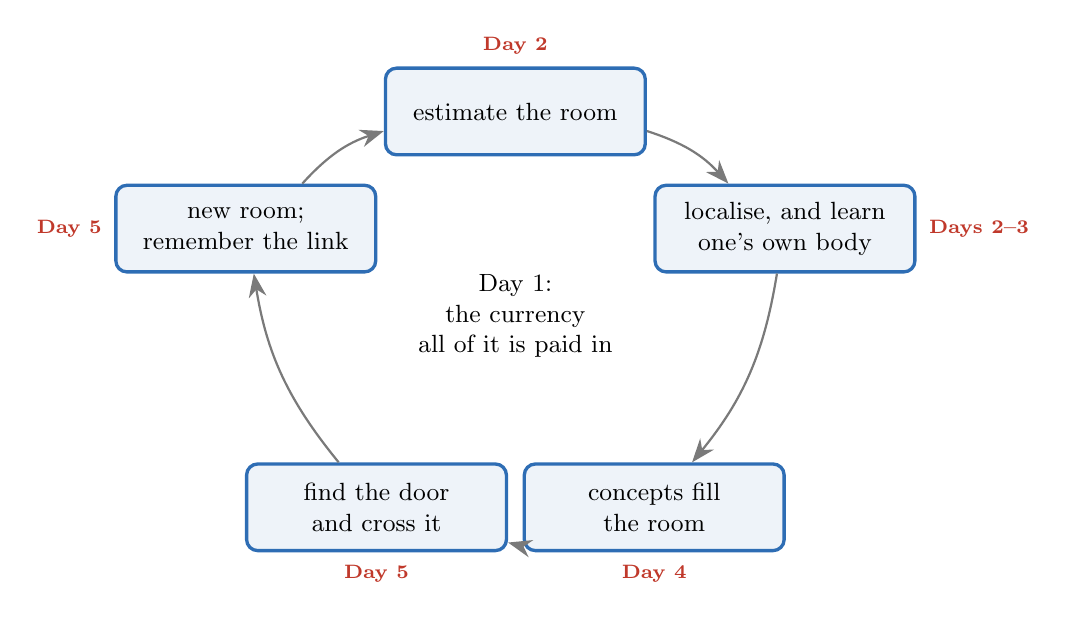
\begin{tikzpicture}[
      stage/.style={draw=cool, very thick, rounded corners=4pt, fill=cool!8, align=center,
                    minimum width=3.3cm, minimum height=1.1cm, font=\small},
      day/.style={font=\scriptsize\bfseries, text=accent},
      arr/.style={-{Stealth[length=3mm]}, thick, color=muted}]
    \node[stage] (room) at (90:2.6)   {estimate the room};
    \node[stage] (loc)  at (18:3.6)   {localise, and learn\\one's own body};
    \node[stage] (obj)  at (-54:3.0)  {concepts fill\\the room};
    \node[stage] (door) at (-126:3.0) {find the door\\and cross it};
    \node[stage] (mem)  at (162:3.6)  {new room;\\remember the link};
    \draw[arr] (room) to[bend left=15] (loc);
    \draw[arr] (loc)  to[bend left=15] (obj);
    \draw[arr] (obj)  to[bend left=15] (door);
    \draw[arr] (door) to[bend left=15] (mem);
    \draw[arr] (mem)  to[bend left=15] (room);
    \node[day, above=1pt of room] {Day 2};
    \node[day, right=1pt of loc]  {Days 2--3};
    \node[day, below=1pt of obj]  {Day 4};
    \node[day, below=1pt of door] {Day 5};
    \node[day, left=1pt of mem]   {Day 5};
    \node[align=center, font=\small] at (0,0) {Day 1:\\the currency\\all of it is paid in};
  \end{tikzpicture}
\end{frame}

\begin{frame}{Every stage is a belief}
  \footnotesize
  \begin{tabular}{@{}l l l c@{}}
    \toprule
    stage & what is unknown (latent) & what supplies the evidence & day \\
    \midrule
    estimate the room   & walls, corners, the polygon            & LiDAR returns                     & 2 \\
    localise            & the robot's pose in that room          & LiDAR against the believed room   & 2 \\
    learn the body      & wheel scale, gyro bias, sensor mounts  & the localiser's corrections       & 3 \\
    concepts            & which objects exist, where, what shape & camera masks, LiDAR               & 4 \\
    door                & where it is, whether it is open        & the room's boundary, free space   & 5 \\
    new room + memory   & a second polygon; how rooms connect    & all of the above, again           & 5 \\
    \bottomrule
  \end{tabular}

  \vspace{1.2em}
  One generative model over all of it, and \alert{one} quantity that every stage minimises:
  perception lowers it by changing beliefs, action by changing the data.
\end{frame}

\begin{frame}{The toy version you will build, one stage a day}
  \centering
  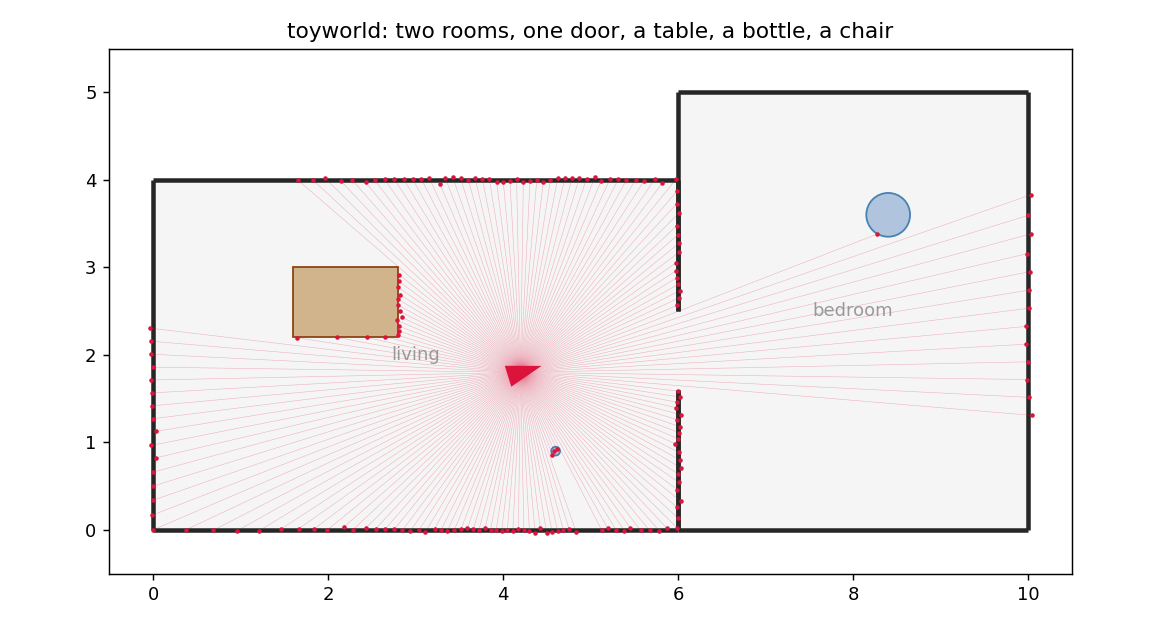
\includegraphics[width=0.78\textwidth]{toyworld.png}

  \small Two rooms, one door, three objects, a LiDAR, and a robot whose wheels lie a little.
  Pure \texttt{numpy}; it runs on your laptop.
\end{frame}

\begin{frame}{How this course is built}
  \begin{columns}[T]
    \begin{column}{0.48\textwidth}
      Each session runs through three steps:
      \begin{enumerate}
        \item the \textbf{theory}, derived rather than asserted;
        \item the \textbf{code}, one stage of the cycle, in the lab;
        \item the \textbf{measurements} that showed when the equations were wrong.
      \end{enumerate}
      \vspace{0.5em}
      The third step is not optional. Most of what the thesis learned, it learned there.
    \end{column}
    \begin{column}{0.48\textwidth}
      \begin{block}{The thread through all five days}
        Averaging removes \alert{independent} error.\\
        It does not remove \alert{shared} error.
      \end{block}
      \small
      You will meet it as:
      \begin{itemize}
        \item the common-mode ceiling;
        \item a prior re-centred on its own estimate;
        \item a fused precision better than its best member;
        \item a metric that scores what the robot never saw.
      \end{itemize}
    \end{column}
  \end{columns}
\end{frame}

% =================================================================================================
\section{The grammar of uncertainty}
% =================================================================================================

\begin{frame}{What the robot is uncertain about}
  \begin{columns}[c]
    \begin{column}{0.5\textwidth}
      \begin{tabular}{@{}l l@{}}
        \toprule
        deterministic & $y = f(x)$: one outcome \\
        random        & $y = f(x) + \varepsilon$: many outcomes \\
        \midrule
        discrete      & a door is open \emph{or} closed \\
        continuous    & a wall is $4.013\ldots$ m away \\
        \bottomrule
      \end{tabular}

      \vspace{1em}
      Everything the robot does not know is a \textbf{random variable}, and what it believes about
      it is a \textbf{probability distribution}: a table for discrete variables, a density for
      continuous ones.
    \end{column}
    \begin{column}{0.46\textwidth}
      \small
      \[
        s = \begin{bmatrix} x\\ y\\ \theta\\ w\\ d \end{bmatrix}\!
        \begin{array}{l}\text{robot pose}\\[0.2em] \text{room width, depth}\end{array}
      \]
      \[
        o = \begin{bmatrix} p_1\\ \vdots\\ p_N \end{bmatrix}\! \text{ LiDAR returns}
        \quad
        a = \begin{bmatrix} v_{\text{adv}}\\ v_{\text{side}}\\ \omega \end{bmatrix}\! \text{ command}
      \]
      The whole problem is one object:
      \[ p(s, o, a) \]
    \end{column}
  \end{columns}
\end{frame}

\begin{frame}{The joint distribution: everything there is to know}
  A two-variable world. $D$: is the door open? $O$: does the LiDAR see a gap where the door is?
  \vspace{0.6em}
  \begin{columns}[c]
    \begin{column}{0.45\textwidth}
      \centering
      \renewcommand{\arraystretch}{1.3}
      \begin{tabular}{@{}l|cc@{}}
                            & $O=\text{gap}$ & $O=\text{wall}$ \\ \hline
        $D=\text{open}$     & 0.27 & 0.03 \\
        $D=\text{closed}$   & 0.14 & 0.56 \\
      \end{tabular}

      \vspace{0.5em}
      {\small the four numbers add up to 1}
    \end{column}
    \begin{column}{0.52\textwidth}
      \begin{itemize}
        \item The \textbf{joint} $p(D, O)$ gives the probability of every combination at once.
        \item Every question you can ask about $D$ and $O$ is a calculation on this table, with
              only \alert{three operations}: summing, slicing, and multiplying back.
        \item Everything this week, including free energy, is these three operations, done on
              tables too large to write down.
      \end{itemize}
    \end{column}
  \end{columns}
\end{frame}

\begin{frame}{Marginalisation: sum out what you do not care about}
  \begin{columns}[c]
    \begin{column}{0.5\textwidth}
      \centering
      \renewcommand{\arraystretch}{1.3}
      \begin{tabular}{@{}l|cc|>{\columncolor{cool!12}}c@{}}
                            & gap  & wall & $p(D)$ \\ \hline
        open                & 0.27 & 0.03 & 0.30 \\
        closed              & 0.14 & 0.56 & 0.70 \\ \hline
        \rowcolor{good!12}
        $p(O)$              & 0.41 & 0.59 & 1 \\
      \end{tabular}
    \end{column}
    \begin{column}{0.48\textwidth}
      \[ p(o) = \sum_{d} p(d, o) \qquad p(o) = \int p(s, o)\,\mathrm{d}s \]
      \begin{itemize}\small
        \item Sum each row or column and write the result \emph{in the margin}: that is where
              the name comes from.
        \item A marginal answers a question about one variable while staying honest about
              every value the other one might take.
        \item The integral over $s$ is the expensive one. Remember it.
      \end{itemize}
    \end{column}
  \end{columns}
\end{frame}

\begin{frame}{Conditioning: keep the slice you observed, renormalise}
  \begin{columns}[c]
    \begin{column}{0.5\textwidth}
      \centering
      \renewcommand{\arraystretch}{1.3}
      \begin{tabular}{@{}l|>{\columncolor{accent!12}}c c@{}}
                            & gap  & wall \\ \hline
        open                & 0.27 & 0.03 \\
        closed              & 0.14 & 0.56 \\ \hline
        $p(O)$              & 0.41 & 0.59 \\
      \end{tabular}

      \vspace{0.8em}
      \[ p(\text{open}\given\text{gap}) = \frac{0.27}{0.41} = 0.66 \]
    \end{column}
    \begin{column}{0.48\textwidth}
      \[ p(s\given o) = \frac{p(s, o)}{p(o)} \]
      \begin{itemize}\small
        \item Observing $O=\text{gap}$ throws away the column that did not happen. What remains
              no longer sums to 1, so divide by its total, the marginal $p(o)$.
        \item Before looking, the door was open with probability $0.30$; after seeing a gap,
              $0.66$. \alert{Conditioning is how evidence enters a belief.}
        \item Seeing a wall instead: $0.03/0.59 = 0.05$.
      \end{itemize}
    \end{column}
  \end{columns}
\end{frame}

\begin{frame}{Factorisation: the product rule}
  Turn the conditioning formula around:
  \[
    p(s, o) \;=\; \underbrace{p(o\given s)\,p(s)}_{\text{first $s$, then $o$ given $s$}}
            \;=\; \underbrace{p(s\given o)\,p(o)}_{\text{first $o$, then $s$ given $o$}}
  \]
  \vspace{-0.3em}
  \begin{columns}[T]
    \begin{column}{0.5\textwidth}
      Check it on the table:
      \begin{itemize}\small
        \item $p(\text{gap}\given\text{open})\,p(\text{open}) = 0.9 \times 0.30 = 0.27$
        \item $p(\text{open}\given\text{gap})\,p(\text{gap}) = 0.66 \times 0.41 = 0.27$
      \end{itemize}
      Both products rebuild the same cell of the joint.
    \end{column}
    \begin{column}{0.46\textwidth}
      Set the two factorisations equal and divide by $p(o)$:
      \[ p(s\given o) = \frac{p(o\given s)\,p(s)}{p(o)} \]
      \alert{Bayes' rule is not an extra axiom.} It is the product rule written twice.
    \end{column}
  \end{columns}
\end{frame}

\begin{frame}{The same operations on continuous variables}
  \begin{columns}[c]
    \begin{column}{0.56\textwidth}
      \centering
      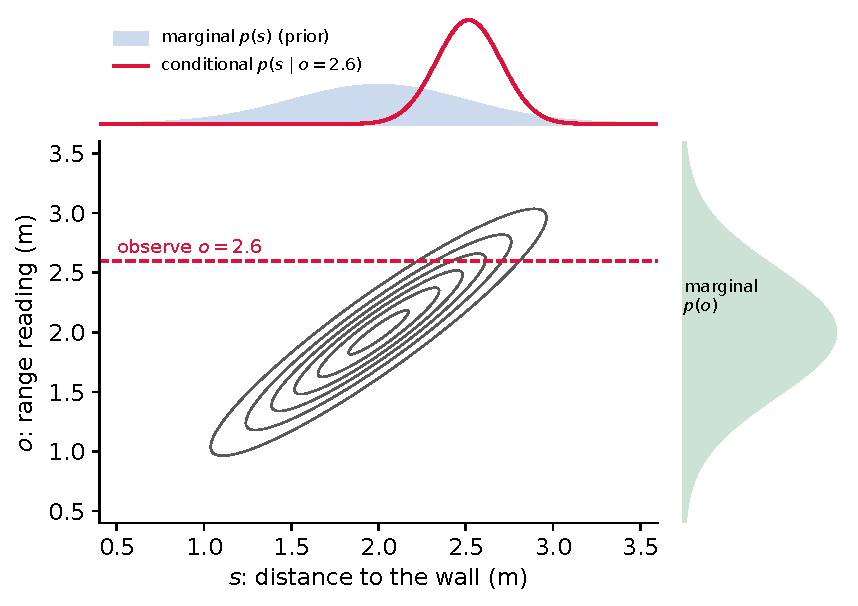
\includegraphics[width=\textwidth]{d1_gaussian_ops.pdf}
    \end{column}
    \begin{column}{0.42\textwidth}
      \small
      $s$: distance to a wall, prior $\N(2,\,0.5^2)$.\\
      $o$: its range reading, $o\given s \sim \N(s,\,0.2^2)$.
      \begin{itemize}
        \item The \textbf{joint} is the tilted ellipse: readings track distances.
        \item A \textbf{marginal} is the shadow the joint casts on one axis.
        \item A \textbf{conditional} is one horizontal cut through it, rescaled to area 1.
      \end{itemize}
      Reading $o = 2.6$ moves the belief from $2.00 \pm 0.50$ to $2.52 \pm 0.19$ m.
    \end{column}
  \end{columns}
  \src{figures/make\_day1.py, block 6}
\end{frame}

\begin{frame}{For Gaussians, both operations are linear algebra}
  Split a Gaussian over $(s, o)$ into blocks, written two ways:
  \[
    \text{covariance } \Sigma = \begin{bmatrix} \Sigma_{ss} & \Sigma_{so}\\ \Sigma_{os} & \Sigma_{oo} \end{bmatrix}
    \qquad
    \text{precision } \Lambda = \Sigma^{-1} = \begin{bmatrix} \Lambda_{ss} & \Lambda_{so}\\ \Lambda_{os} & \Lambda_{oo} \end{bmatrix}
  \]
  \begin{center}
  \renewcommand{\arraystretch}{1.4}
  \begin{tabular}{@{}l c c@{}}
    \toprule
                         & in covariance form & in precision form \\
    \midrule
    marginalise out $o$  & keep the block: $\Sigma_{ss}$ & Schur complement: $\Lambda_{ss} - \Lambda_{so}\Lambda_{oo}^{-1}\Lambda_{os}$ \\
    condition on $o$     & Schur complement: $\Sigma_{ss} - \Sigma_{so}\Sigma_{oo}^{-1}\Sigma_{os}$ & keep the block: $\Lambda_{ss}$ \\
    \bottomrule
  \end{tabular}
  \end{center}
  \begin{itemize}\small
    \item Each form makes one operation free and the other costly. The slide before:
          $0.25 - 0.25^2/0.29 = 0.035 = 0.19^2$.
    \item The robot keeps its beliefs in precision form. When it forgets an old pose (Days 2--5),
          it is marginalising, and it pays a Schur complement.
  \end{itemize}
\end{frame}

\begin{frame}{The chain rule: $N$ variables, $N$ factors}
  Apply the product rule again and again, peeling off one variable each time:
  \begin{align*}
    p(A, B)       &= p(A\given B)\,p(B) \\
    p(A, B, C)    &= p(A\given B, C)\,p(B\given C)\,p(C) \\
    p(A, B, C, D) &= p(A\given B, C, D)\,p(B\given C, D)\,p(C\given D)\,p(D)
  \end{align*}
  In general, for any ordering $\pi$ of the variables:
  \[
    p(X_1, \ldots, X_N) =
    \underbrace{p(X_{\pi(1)})\,p(X_{\pi(2)}\given X_{\pi(1)})\cdots
                p(X_{\pi(N)}\given X_{\pi(1)}, \ldots, X_{\pi(N-1)})}_{N\text{ factors}}
  \]
  \begin{itemize}\small
    \item No assumption was made. This is exact for every distribution.
    \item But the last factor depends on everything: nothing has been gained yet.
  \end{itemize}
\end{frame}

\begin{frame}{One joint, $N!$ factorisations}
  From now on the names we use all week: $S$ the \textbf{state} (is the door open?),
  $O$ the \textbf{observation} (does the LiDAR see a gap?), $A$ the \textbf{action} (does the
  robot turn its LiDAR towards the door, or away?).
  \vspace{0.3em}
  \begin{columns}[c]
    \begin{column}{0.5\textwidth}
      \small
      \begin{align*}
        p(S,O,A) &= p(S)\,p(O\given S)\,p(A\given S,O)\\
                 &= p(S)\,p(A\given S)\,p(O\given S,A)\\
                 &= p(O)\,p(S\given O)\,p(A\given S,O)\\
                 &= p(O)\,p(A\given O)\,p(S\given O,A)\\
                 &= p(A)\,p(S\given A)\,p(O\given S,A)\\
                 &= p(A)\,p(O\given A)\,p(S\given O,A)
      \end{align*}
    \end{column}
    \begin{column}{0.46\textwidth}
      \begin{itemize}
        \item 3 variables give $3! = 6$ orderings, each with 3 factors.
        \item $N$ variables give $N!$. A robot tracked over 100 steps has hundreds of
              variables.
        \item All of them are \alert{exactly equal}. No amount of data can tell them apart.
      \end{itemize}
      \vspace{0.3em}
      So which one do we write down?
    \end{column}
  \end{columns}
\end{frame}

\begin{frame}{Choose the order in which the world produces things}
  \begin{columns}[T]
    \begin{column}{0.5\textwidth}
      \textbf{Causal order}: causes before effects.
      \[ p(S)\,p(A\given S)\,p(O\given S, A) \]
      The robot cannot see whether the door is open, so where it points its LiDAR does not
      depend on it; what it observes depends on both:
      \[ p(A\given S) = p(A) \]
      \centering
      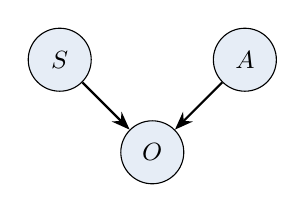
\begin{tikzpicture}[v/.style={draw, circle, minimum size=0.8cm, fill=cool!12}, every node/.style={font=\small}]
        \node[v] (o) {$O$};
        \node[v, above left=0.6cm and 0.6cm of o] (s) {$S$};
        \node[v, above right=0.6cm and 0.6cm of o] (a) {$A$};
        \draw[-{Stealth}, thick] (s) -- (o);
        \draw[-{Stealth}, thick] (a) -- (o);
      \end{tikzpicture}
    \end{column}
    \begin{column}{0.48\textwidth}
      \textbf{Anti-causal order}: effects first.
      \[ p(O)\,p(A\given O)\,p(S\given O, A) \]
      Once $O$ is known, $S$ and $A$ are linked through it (a gap means little if the LiDAR
      looked away), so nothing simplifies. Every factor keeps all its arguments.

      \vspace{0.6em}
      \footnotesize
      Numbers needed to specify it (binary variables):\\[0.3em]
      \begin{tabular}{@{}l r@{}}
        \toprule
        any order, nothing dropped         & $2^3 - 1 = 7$ \\
        causal, using $A \perp S$          & $1 + 1 + 4 = 6$ \\
        \midrule
        $N$ variables, any order           & $2^N - 1$ \\
        $N$ variables, $\le k$ causes each & $\le N\,2^k$ \\
        \bottomrule
      \end{tabular}
    \end{column}
  \end{columns}
\end{frame}

\begin{frame}{Why the causal order wins}
  \begin{enumerate}
    \item \textbf{Sparse.} Each variable depends on a few direct causes, not on everything
          before it. The arrows you leave out are the independences you know.
    \item \textbf{Each factor is a piece of physics.} $p(O\given S, A)$ is a sensor model and
          $p(s_t\given s_{t-1}, a_t)$ a motion model; you can write them down. Nobody can write
          down $p(O)$, the distribution of every possible LiDAR scan.
    \item \textbf{Modular.} Replace the LiDAR with a camera and only $p(O\given S, A)$ changes.
          In the anti-causal order, all three factors change.
    \item \textbf{It runs forwards.} Sampling the factors in order \emph{generates} data: the
          model can predict what it will see if it acts. Action needs exactly that.
  \end{enumerate}
\end{frame}

\begin{frame}{Three things you can build from one joint}
  \begin{columns}[T]
    \begin{column}{0.31\textwidth}
      \begin{block}{Perception only}
        \centering $p(s\given o)$\\[0.3em]
        \raggedright\small From an image, guess the state: a classifier, a detector.\\[0.3em]
        It answers one question, in one direction.
      \end{block}
    \end{column}
    \begin{column}{0.31\textwidth}
      \begin{block}{Control only}
        \centering $p(a\given o)$\\[0.3em]
        \raggedright\small From an observation, choose the action: a PID loop, a hand-written
        controller, a policy learnt by reinforcement.\\[0.3em]
        It is the factor $p(A\given O)$ of the anti-causal order, used on its own.
      \end{block}
    \end{column}
    \begin{column}{0.31\textwidth}
      \begin{exampleblock}{The generative model}
        \centering $p(s)\,p(a)\,p(o\given s, a)$\\[0.3em]
        \raggedright\small Explain what is seen, predict what each action would show, and
        choose the action by inference.\\[0.3em]
        This is what we build.
      \end{exampleblock}
    \end{column}
  \end{columns}
  \vspace{0.6em}
  \small
  A controller or a learnt policy can act very well, in the world it was tuned or trained in.
  What it cannot do is say what it expects to see, notice that it is surprised, tell what it does
  not know, or survive a sensor swap without being re-tuned: none of that is in $p(a\given o)$.
  \alert{Every one of those is a question the joint can answer.}
\end{frame}

\begin{frame}{The robot's joint, in causal order}
  \centering
  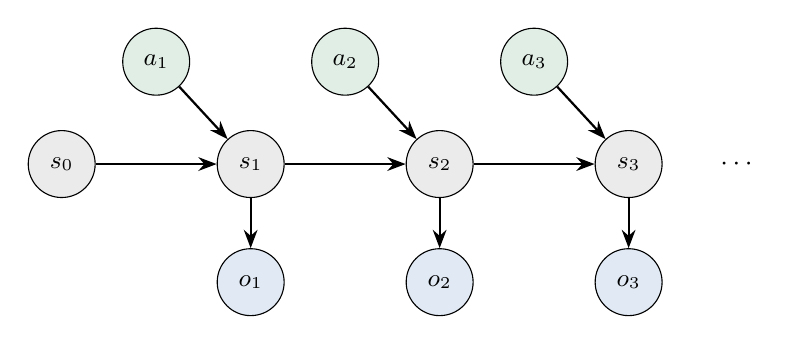
\begin{tikzpicture}[
      v/.style={draw, circle, minimum size=0.85cm, font=\small},
      s/.style={v, fill=muted!15}, o/.style={v, fill=cool!15}, a/.style={v, fill=good!15},
      arr/.style={-{Stealth}, thick}]
    \foreach \t/\x in {0/0, 1/2.4, 2/4.8, 3/7.2} {
      \node[s] (s\t) at (\x, 0) {$s_{\t}$};
    }
    \foreach \t/\x in {1/2.4, 2/4.8, 3/7.2} {
      \node[o] (o\t) at (\x, -1.5) {$o_{\t}$};
      \node[a] (a\t) at (\x - 1.2, 1.3) {$a_{\t}$};
      \draw[arr] (s\t) -- (o\t);
      \draw[arr] (a\t) -- (s\t);
    }
    \draw[arr] (s0) -- (s1); \draw[arr] (s1) -- (s2); \draw[arr] (s2) -- (s3);
    \node at (8.6, 0) {$\cdots$};
  \end{tikzpicture}
  \[
    p(s_{0:T}, o_{1:T}, a_{1:T}) =
    \underbrace{p(s_0)}_{\text{prior}}\;
    \prod_{t=1}^{T}
    \underbrace{p(a_t)}_{\text{policy}}\,
    \underbrace{p(s_t\given s_{t-1}, a_t)}_{\text{motion model}}\,
    \underbrace{p(o_t\given s_t)}_{\text{sensor model}}
  \]
  \small
  $(3T+1)!$ orderings are available, and we write one: each factor touches at most three
  variables and is a piece of physics. This is the \textbf{generative model}; on Day 2 it becomes
  the factor graph the robot actually solves.
\end{frame}

\begin{frame}{Bayes' rule is the three operations in a row}
  \[
    \underbrace{p(s\given o)}_{\text{posterior}}
    \;=\;
    \frac{\overbrace{p(o\given s)}^{\text{likelihood}}\;\overbrace{p(s)}^{\text{prior}}}
         {\underbrace{p(o)}_{\text{evidence}}}
  \]
  \begin{tabular}{@{}l l l@{}}
    \toprule
    operation & where & what it asks \\
    \midrule
    factorise, causally & numerator   & how would a robot at $s$ see this room? what did it expect? \\
    condition on $o$    & left side   & where is the robot, now that this scan has arrived? \\
    marginalise $s$     & denominator & how likely was this scan, averaged over every $s$? \\
    \bottomrule
  \end{tabular}

  \vspace{0.8em}
  \lesson{The first two are cheap. The third is where exact inference dies,\\and the rest of
  today is about how not to compute it.}
\end{frame}

% =================================================================================================
\section{Inference behind a sensory boundary}
% =================================================================================================

\begin{frame}{The agent never sees the state}
  \begin{columns}[c]
    \begin{column}{0.45\textwidth}
      \centering
      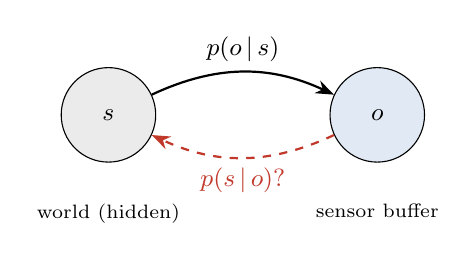
\begin{tikzpicture}[node distance=1.6cm, every node/.style={font=\small}]
        \node[draw, circle, minimum size=1.2cm, fill=muted!15] (s) {$s$};
        \node[draw, circle, minimum size=1.2cm, right=2.2cm of s, fill=cool!15] (o) {$o$};
        \draw[-{Stealth}, thick] (s) to[bend left=25] node[above] {$p(o\given s)$} (o);
        \draw[-{Stealth}, thick, accent, dashed] (o) to[bend left=25] node[below] {$p(s\given o)$?} (s);
        \node[below=0.4cm of s, align=center, font=\scriptsize] {world (hidden)};
        \node[below=0.4cm of o, align=center, font=\scriptsize] {sensor buffer};
      \end{tikzpicture}
    \end{column}
    \begin{column}{0.52\textwidth}
      The \textbf{generative model}:
      \[ p(s,o) = p(o\given s)\,p(s) \]
      \begin{itemize}\small
        \item $p(o\given s)$ is the agent's theory of its own sensor: which LiDAR returns a robot at
              this pose, in this room, would produce.
        \item $p(s)$ is what it brought with it: plausible room shapes, typical table sizes.
      \end{itemize}
      Inference runs the arrow backwards:
      \[ p(s\given o) = \frac{p(o\given s)\,p(s)}{p(o)} \]
    \end{column}
  \end{columns}
  \src{active\_inference.tex l.181--212}
\end{frame}

\begin{frame}{Where exact inference dies}
  \[ p(o) = \int p(o\given s)\,p(s)\,\mathrm{d}s \]
  \begin{itemize}
    \item The probability of \emph{this scan} under \emph{every} room and furniture configuration
          the robot considers possible, each weighted by how likely it is.
    \item No closed form and no feasible quadrature. This is not a quirk of one sensor: it is the
          generic situation.
    \item Every practical method from here on is a way of \alert{not computing it}.
  \end{itemize}
  \vspace{0.8em}
  \begin{block}{A word about ``state''}
    $s$ is a latent variable of the \emph{agent's model}, not the physical truth, which is never
    accessible. That distinction is what gives the question ``is this belief wrong?'' its meaning.
  \end{block}
  \src{active\_inference.tex l.200--220}
\end{frame}

% =================================================================================================
\section{Variational free energy}
% =================================================================================================

\begin{frame}{Do not compute the posterior; approximate it}
  Choose a tractable family, and a member $q(s)$ of it (the \textbf{belief}). Move it towards
  the true posterior, measuring closeness by
  \[ \KL{q(s)}{p(s\given o)} = \int q(s) \ln\frac{q(s)}{p(s\given o)}\,\mathrm{d}s \;\ge 0 . \]
  \pause
  \alert{Problem:} it contains $p(s\given o)$, the very thing we cannot have.

  \pause
  \vspace{0.5em}
  Substitute Bayes' rule and separate out the part that does not depend on $q$:
  \[
    \KL{q}{p(s\given o)} = \underbrace{\int q(s)\ln\frac{q(s)}{p(o,s)}\,\mathrm{d}s}_{F[q,o]} \;+\; \ln p(o)
  \]
  $F$ needs only the belief and the joint $p(o\given s)p(s)$ the agent already wrote down.
  \src{active\_inference.tex l.222--250}
\end{frame}

\begin{frame}{The identity the framework rests on}
  \[ \boxed{\; F[q,o] = \KL{q(s)}{p(s\given o)} - \ln p(o) \;} \]
  \begin{columns}[T]
    \begin{column}{0.48\textwidth}
      \begin{block}{Reading 1: same minimiser}
        $\ln p(o)$ does not depend on $q$. Minimising the computable $F$ minimises the
        uncomputable divergence.
      \end{block}
    \end{column}
    \begin{column}{0.48\textwidth}
      \begin{block}{Reading 2: a bound on surprise}
        $\mathrm{KL}\ge 0$, so $F \ge -\ln p(o)$. Lowering $F$ makes the belief better \emph{and}
        the data less surprising under the agent's own model.
      \end{block}
    \end{column}
  \end{columns}
  \vspace{0.8em}
  If you know machine learning: $-F$ is the \textbf{ELBO}. Maximising the ELBO and minimising free
  energy are the same operation.
  \src{active\_inference.tex l.252--268}
\end{frame}

\begin{frame}{Complexity minus accuracy}
  \[
    F[q,o] = \underbrace{\KL{q(s)}{p(s)}}_{\text{complexity}}
             \;-\; \underbrace{\E_q\!\left[\ln p(o\given s)\right]}_{\text{accuracy}}
  \]
  \begin{itemize}
    \item \textbf{Accuracy} rewards beliefs under which the data are likely. On its own, it would
          adopt any explanation that fits the current scan.
    \item \textbf{Complexity} charges for the distance travelled from the prior: Occam's razor,
          written as a divergence.
    \item Free energy picks the belief that buys the most accuracy for the least departure from
          what was already believed.
  \end{itemize}
  \lesson{One trade, stated once, in nats, for every quantity the agent believes.}
  \src{active\_inference.tex l.288--308}
\end{frame}

\begin{frame}{Worked example: the Kalman update is free-energy minimisation}
  \small
  Take the prior $s\sim\N(m,p)$, an observation $y\sim\N(s,r)$, and the belief $q=\N(\mu,\Sigma)$.
  Every term is a Gaussian expectation:
  \[
    F(\mu,\Sigma) = \frac{(\mu-m)^2+\Sigma}{2p} + \frac{(y-\mu)^2+\Sigma}{2r} - \tfrac12\ln\Sigma + \text{const}
  \]
  \pause
  \begin{columns}[T]
    \begin{column}{0.48\textwidth}
      $\partial F/\partial\mu = 0$:
      \[ \mu = \frac{m/p + y/r}{1/p + 1/r} \]
      the precision-weighted mean.
    \end{column}
    \begin{column}{0.48\textwidth}
      $\partial F/\partial\Sigma = 0$:
      \[ \frac1\Sigma = \frac1p + \frac1r \]
      precisions add.
    \end{column}
  \end{columns}
  \vspace{0.5em}
  \pause
  The two halves come from different terms. The \emph{mean} comes from the prediction errors; the
  \emph{variance} comes from the curvature of $F$ balanced against the entropy
  $-\tfrac12\ln\Sigma$. Regularised least squares is the same trade with a flat prior.
\end{frame}

\begin{frame}{A choice, marked as a choice}
  \begin{itemize}
    \item Closeness was measured with $\mathrm{KL}$. Nothing forced that: it is the $\alpha\to1$
          member of the Rényi family, and the bound survives the substitution.
    \item The order $\alpha$ controls the \emph{character} of the error: does the belief err
          towards too broad, or towards too confident?
    \item On this robot, that is not a statistical nicety. A covariance is \alert{spent}: on
          deciding where to look next, and on how far a measurement may move a belief.
  \end{itemize}
  \vspace{0.5em}
  The thesis keeps $\alpha\to1$ throughout. Making $\alpha$ itself a latent variable is open
  future work.
  \src{active\_inference.tex l.270--286; future\_work.tex l.22}
\end{frame}

% =================================================================================================
\section{The Laplace approximation}
% =================================================================================================

\begin{frame}{Gaussian beliefs: the form everything later takes}
  Take $q(s)=\N(\mu,\Sigma)$ and expand around the mode:
  \[
    F \approx -\ln p(o,\mu) + \tfrac12\operatorname{tr}(\Hess\Sigma) - \tfrac12\ln|\Sigma| - \tfrac n2\ln(2\pi e),
    \qquad \Hess = -\nabla^2_s \ln p(o,s)\big|_{\mu}
  \]
  \begin{itemize}
    \item The \textbf{mean} moves to the mode of the joint: a nonlinear least-squares problem
          (Gauss--Newton).
    \item The \textbf{covariance} is pulled two ways: the curvature term shrinks it, the entropy
          term widens it. Setting $\partial F/\partial\Sigma=0$:
  \end{itemize}
  \[ \boxed{\;\Sigma = \Hess^{-1}\;} \]
  \lesson{The uncertainty comes as a by-product of fitting, at no extra modelling cost.}
  \src{active\_inference.tex l.310--333}
\end{frame}

\begin{frame}{Gauss--Newton, in one line}
  For whitened residuals $r(s)$ with noise covariance $R$, and a Gaussian prior $\N(m,P)$:
  \[
    -\ln p(o,s) = \tfrac12 r^\top R^{-1} r + \tfrac12 (s-m)^\top P^{-1}(s-m) + \text{const},
  \]
  \[
    \Hess \approx J^\top R^{-1} J + P^{-1}, \qquad
    \Delta s = -\Hess^{-1}\big(J^\top R^{-1} r + P^{-1}(s-m)\big).
  \]
  \begin{itemize}
    \item Iterate to convergence. The final $\Hess^{-1}$ \emph{is} the belief's covariance.
    \item In the lab, \texttt{laplace(residual, x0, sigma, prior=...)} does exactly this. It also
          returns the Laplace free energy
          $F \approx -\ln p(o,\mu) + \tfrac12\ln|\Hess| - \tfrac n2\ln 2\pi$,
          which you will use to compare models.
  \end{itemize}
\end{frame}

\begin{frame}{Example: one wall as a belief}
  \begin{columns}[c]
    \begin{column}{0.55\textwidth}
      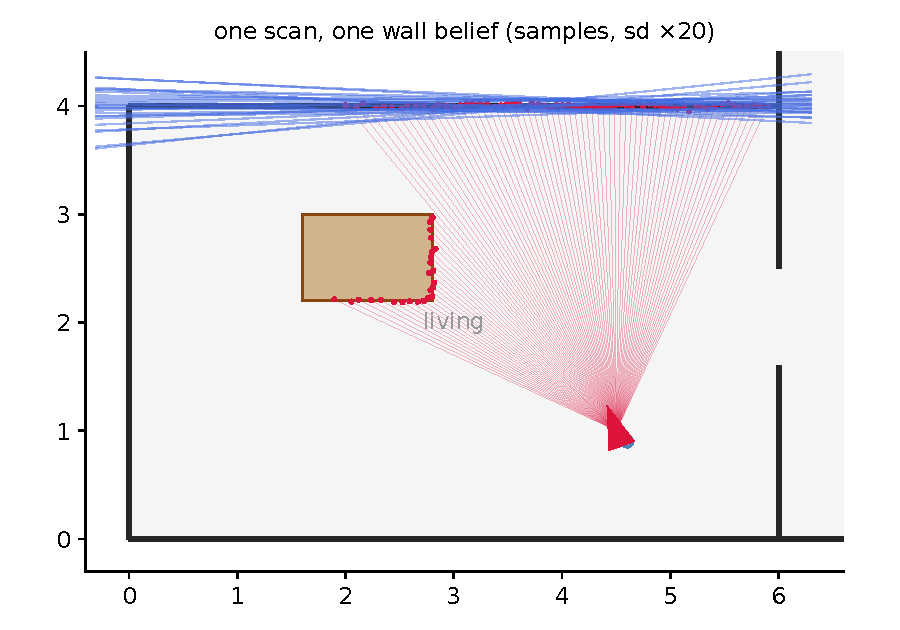
\includegraphics[width=\textwidth]{d1_wall_belief.pdf}
    \end{column}
    \begin{column}{0.43\textwidth}
      \small
      A line with normal $n(\alpha)$ at distance $d$:
      \[ r_i = \cos\alpha\,x_i + \sin\alpha\,y_i - d \]
      \[ \frac{\partial r_i}{\partial(\alpha,d)} = \big[\,-\sin\alpha\,x_i + \cos\alpha\,y_i,\; -1\,\big] \]
      \begin{itemize}
        \item The first column is a \textbf{lever arm}. Points far apart along the wall pin the
              angle.
        \item $\alpha$ and $d$ come out correlated ($\rho\approx-0.97$), because $d$ is measured
              from an origin the points are far away from.
      \end{itemize}
    \end{column}
  \end{columns}
\end{frame}

\begin{frame}{Is the covariance honest?}
  \begin{columns}[c]
    \begin{column}{0.45\textwidth}
      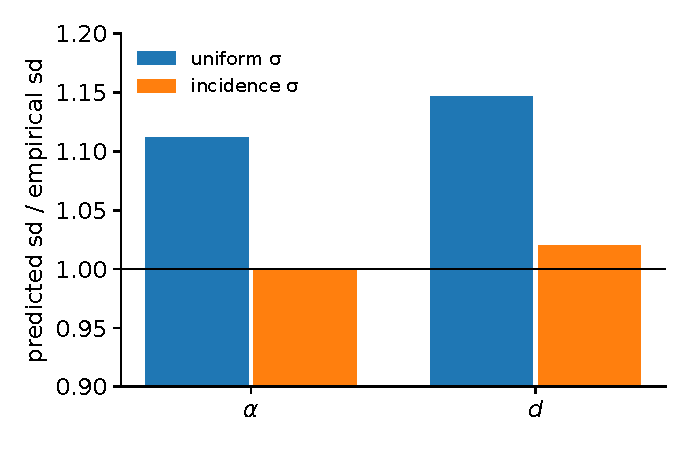
\includegraphics[width=\textwidth]{d1_honesty.pdf}
    \end{column}
    \begin{column}{0.53\textwidth}
      \small
      $\Sigma=\Hess^{-1}$ is a \emph{claim} about how far the fit would move on a re-scan.
      Test it with 400 scans from one pose:
      \begin{itemize}
        \item uniform $\sigma$: about 10\% too pessimistic, and it does not average away;
        \item the noise is along the \emph{beam}, the residual along the wall's \emph{normal}:
              $\sigma_i=\sigma\,|u_i^\top n|$;
        \item with that likelihood: within a few per cent.
      \end{itemize}
    \end{column}
  \end{columns}
  \lesson{A Laplace covariance is exactly as honest as the likelihood you wrote.}
  \src{lab 1, exercises 3--4; the real localiser's incidence weight: room\_concept.tex l.232}
\end{frame}

\begin{frame}{Free energy compares models: the price of a parameter}
  \begin{columns}[c]
    \begin{column}{0.45\textwidth}
      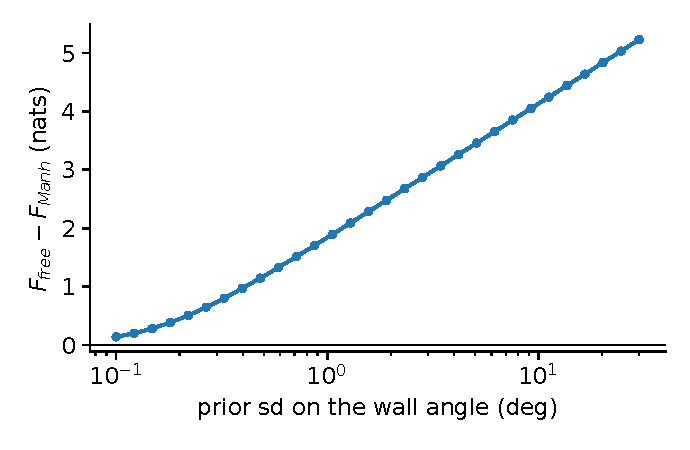
\includegraphics[width=\textwidth]{d1_occam.pdf}
    \end{column}
    \begin{column}{0.53\textwidth}
      \small
      Two models of the same wall:
      \begin{itemize}
        \item \textbf{Manhattan}: the angle is fixed at $90^\circ$; one parameter, $d$.
        \item \textbf{free}: $\alpha\sim\N(90^\circ,s^2)$; two parameters.
      \end{itemize}
      Both fit equally well. The free model pays
      $\approx\ln(s/\sigma_\alpha)$ nats of \emph{complexity}: the cost of squeezing the prior
      down to the posterior.\\[0.4em]
      Tilt the points by $1.5^\circ$ and the verdict flips by \alert{70 nats}.
    \end{column}
  \end{columns}
  \lesson{Nobody wrote ``if the angle error exceeds $k$ degrees''. That is the first instance of
          \textbf{no thresholds}.}
\end{frame}

% =================================================================================================
\section{What measurement said}
% =================================================================================================

\begin{frame}{Free energy is not computation}
  \begin{measured}{a better model does not save arithmetic}
    Injecting a body-model error from 0 to 10\%:
    \begin{itemize}
      \item the solver iterations per correction stay flat to within a twentieth;
      \item the size of the correction grows by about half as much again.
    \end{itemize}
  \end{measured}
  \begin{itemize}
    \item The agent pays in \emph{how far its beliefs must move}. The arithmetic doing the moving
          is nearly constant.
    \item ``A better model saves the agent work'' has to say \emph{which} work. The two readings
          come apart, and an endpoint chosen on the wrong reading measures nothing.
  \end{itemize}
  \src{active\_inference.tex l.835--848}
\end{frame}

\begin{frame}{A factor inherits the errors of what it is estimated through}
  \begin{columns}[T]
    \begin{column}{0.52\textwidth}
      \begin{itemize}
        \item The body is learnt from the localiser's corrections, which are fitted against the
              room. So a wrong map is charged to the wheels.
        \item \alert{A robot in a room whose map is wrong will conclude that its wheels are
              wrong.}
        \item And it gets \emph{quieter}, not louder: once the body has absorbed the map's
              distortion, the two agree. The state is internally consistent and externally wrong.
      \end{itemize}
    \end{column}
    \begin{column}{0.45\textwidth}
      \begin{measured}{an omitted parameter}
        Admitting a camera-mount translation the data cannot support moves the reported pitch by
        \textbf{nine times} its stated interval. An interval speaks only about the parameters the
        model contains.
      \end{measured}
    \end{column}
  \end{columns}
  \lesson{Carry an external reference. Never trust only what the agent computes about itself.}
  \src{active\_inference.tex l.899--950}
\end{frame}

% =================================================================================================
\section{Lab}
% =================================================================================================

\begin{frame}{Lab 1: probability by hand, then a wall as a belief}
  \texttt{labs/day1.ipynb}, about 50 minutes. Today the robot knows its pose and we cheat on which
  points are the wall's.
  \begin{enumerate}\small
    \item \textbf{Warm-up}: the door table by hand (marginalise, condition, both factorisations);
          read an anti-causal order off a joint; condition a Gaussian in both forms.
    \item Write the wall's residual and Jacobian; fit it with \texttt{laplace}.
    \item \textbf{Honesty test}: 500 scans; predicted vs empirical $\sigma$. Find the 10\% and fix
          the likelihood.
    \item \textbf{Model choice}: Manhattan vs free, by $\Delta F$. Then tilt the wall.
  \end{enumerate}
  \vspace{0.4em}
  \small Where to look next waits for Day 3, once action has a functional of its own.
\end{frame}

\begin{frame}{Tomorrow}
  \begin{columns}[c]
    \begin{column}{0.55\textwidth}
      The robot loses both of today's cheats:
      \begin{itemize}
        \item it no longer knows its pose;
        \item it no longer knows which points belong to which wall.
      \end{itemize}
      One wall becomes a room, the pose becomes one more belief, and the two must be estimated
      \emph{together}.\\[0.5em]
      And we measure the common-mode ceiling: how little a thousand points can teach when they
      share one error.
    \end{column}
    \begin{column}{0.4\textwidth}
      \begin{block}{Reading for Day 2}\small
        Thesis chapters:
        \begin{itemize}
          \item \emph{Estimating the Layout of an Unknown Room}, \S\S 1--5;
          \item \emph{The Room Concept Agent}, \S\S ``What is estimated'' and ``The observation
                model''.
        \end{itemize}
      \end{block}
    \end{column}
  \end{columns}
\end{frame}

\end{document}
